
\begin{figure}
  \centering
  \begin{subfigure}[b]{0.45\linewidth}
    \includegraphics[width=\textwidth]{hsp_interface-global.png}
    \caption{Global view}
    \label{fig:interface:global} 
  \end{subfigure} 
  ~
  \begin{subfigure}[b]{0.45\linewidth}
    \includegraphics[width=\textwidth]{hsp_interface-local.png}
    \caption{Local view}
    \label{fig:interface:local} 
  \end{subfigure}
  \caption[The interface for browsing slices created by the Hypersliceplorer algorithm.]{%
    The interface for browsing slices created by the Hypersliceplorer algorithm.
    We show a plot for each pair of dimensions laid out in the same way as
    HyperSlice~\cite{Wijk:1993}.
    The interface has two modes: global and local view.
    The global view (\subref{fig:interface:global}) 
    shows the results of sampling over a number of focus points. The views
    are linked through highlighting a slice. The local view 
    (\subref{fig:interface:local}) shows a single selected slice and then
    the user can add additional slices by clicking the ``+ fp'' button.
  }
  \label{fig:interface}
\end{figure}

One-dimensional slices cannot do everything. When we are examining shapes then
we need to examine the relationship between dimensions. Thus, 2D slices are the
minimum number necessary to examine these relationships (see
\autoref{tbl:task_list}).  If we have a function describing the
multi-dimensional shape we are examining then we can generate two-dimensional
slices by constraining all but two of the parameters to a particular value and
then computing the two-dimensional outline directly. However, there are
domains, such as polytopes, where we have a simplical mesh of the continuous
object. In this case, we cannot use the dimension constraining method. In this
chapter, I develop an algorithm for generating two-dimensional slices of these
multi-dimensional simplical objects. 
This chapter is based on joint work with Torsten M{\"oller}, Michael Sedlmair,
and R. Mike Kirby currently under submission to the 20th EG/VGTC Conference
on Visualization (EuroVis 2018).

%Thesis: Multi-dimensional spaces are better visualized through slice based views

We live in a three-dimensional world.  Ourselves and what we can interact with
are in three dimensions.  We learn about our world by studying the various
phenomena around us.  These phenomena are described as continuous processes.
In the beginning of our  education we study function plots in high school.
These give an intuitive view of one-dimensional phenomena.  By exploring the
relationship between an input factor
and output,
we can build an understanding on the relationship between the two.  We can also
compare one function plot to another. Visual inspection of these plots allows
us to see common patterns. We use our pattern recognition ability to quickly
categorize these different plots into different types of function behavior.
Function plots can also be used to describe two-dimensional phenomena. These
show the effect due to two input factors. In this case we can use the third
dimension or color encoding to show the function value.  From these plots we
can also make general statements about the ``shapes'' of the behavior like how
``peaky'' the function is or if it is monotonically increasing. These shapes
give us intuition into the underlying processes and help us learn about the
world~\cite{Palmer:1999}.

The visual analysis of multiple dimensions is one of the central themes of
visualization research. In principle there are two conceptual types of problems
that amount to two different mental models. (1) Often, the data set is
considered to be truly discrete and projection methods, such as scatterplots
and dimensionality reduction techniques, are used for its analysis.  Typical
examples include business applications, in which one is analyzing customer
data.  The focus of this paper is different in that (2) we are focusing on
continuous multi-dimensional data spaces. For computational purposes, the data
set is then merely a set of points sampled from a continuous phenomenon of
study. This is rather common in simulation and engineering applications or for
the study of continuous algorithmic parameters in modeling environments,
including machine learning applications~\cite{Sedlmair:2014}. Of course, for
such scenarios, projection based visualization might be of help as well.
However, they do not respect the mental model of the object of
study~\cite{Tory:2004}.

Understanding multi-dimensional continuous spaces is difficult. As
three-dimensional beings we have real-world analogs for measurement, angle, and
position in three dimensions. We do not have these once we move beyond three
dimensions though. Nevertheless, visual analysis of these multi-dimensional
spaces has produced insights about the underlying
behavior~\cite{Sedlmair:2014,Gleicher:2016}. The issue is how to show more than
three dimensions on a two-dimensional screen. 

Visualizations of multi-dimensional spaces on a 2D screen must contend with
some sort of reduction of the information. A proper visualization must select
visual encodings that highlight the information we want to see. Any sort of
data reduction requires trade-offs. The best visualization choices acknowledge
any deficiencies to a particular visual encoding. By acknowledging these
deficiencies, we can design tools to compensate for their shortcomings while
still maintaining their advantages. 

Van Wijk and
van Liere introduced the idea of using slice-based views of multi-dimensional
data, called HyperSlice~\cite{Wijk:1993}.
Slicing offers a number of advantages over other multi-dimensional
visualization techniques. Slicing is a direct visualization of the
multi-dimensional object. In contrast to methods like projection or dimension
reduction, slicing does not distort the dimensions in order to display them on
a two-dimensional screen. Since there is no distortion, distances in the visual
representation are directly proportional to distances in the object. 

However, they did not expand on what data types and tasks are involved
in multi-dimensional continuous data analysis.  I investigate
the usefulness of slice-based views of continuous
multi-dimensional datasets. I also identified tasks involved in
multi-dimensional data analysis. The task analysis informed the development of
one- and two-dimensional slice-based views.

\subsection{Multi-dimensional spaces}
\label{sec:motivation:multi-d}

There are a number of domains where one can apply the analysis of continuous
multi-dimensional data.  As of yet, there has not been a comprehensive data and
task analysis for multi-dimensional continuous data analysis. For discrete
data, there are several task 
analyses~\cite{Shneiderman:1996,Brehmer:2013,Amar:2004}. 
However, they are
focused on identifying and selecting particular data items. Continuous datasets
consist of ranges of values as well as functions. Functions can be seen as a
mapping from ranges of numbers to other ranges. The analysis task here is to
study these ranges, their relationships to each other, and the mappings between
them. Tasks addressing these
have not yet been covered by visualization task analyses. Thus,
there is no comprehensive source for what analysis tasks one wants to perform
given a continuous multi-dimensional dataset.  Work in this area has
traditionally focused on developing a specific visualization for a specific
task. For example, topological spines extracts critical points from a scalar
field~\cite{Correa:2011}. One goal of this thesis is to develop this task
taxonomy for visualization of continuous multi-dimensional data.


These domains can be broadly classified into two types based on their analysis
tasks. One type, \emph{manifold} analysis, deals with understanding the
relationship between inputs and outputs. This is a functional relationship.
The user wants to inspect how changes in the inputs (independent variables)
affect the outputs (dependent variables). One can also perform \emph{shape}
analysis. Here, in terms of the analysis tasks, there is no identification of
independent and dependent variables. We look at each of these two in turn.

\subsection{Manifolds}
\label{sec:manifolds}

Studying the mapping between continuous ranges means studying functional
relationships and thus manifolds.  The critical issue is understanding the
relationship between independent and dependent variables.  Subtasks in manifold
analysis include examining critical points, assessing the sensitivity of
parameters, and understanding the shape of the manifold.  
One area where
understanding the manifold is important is analyzing optimization surfaces and
functions.  In this case, the identification of extrema is important for
understanding how many and the relative location of local optima. In addition,
we want to understand the degree to which these are extrema. These can result
in global optimization algorithms ``getting stuck'' in local optima rather than
continuing to search for the global optimum. Optimization algorithms need to be
carefully tuned to properly detect these features and ignore them where
necessary.

Simulations can be used to run experiments that are impractical or impossible
in the real world.  Simulation analysis is another area where the analysis
tasks, in the abstract, are examining functions. If we look back at the weather
simulation from before, the inputs to the function are things like the
temperature and pressure.  The output is, for example, the likelihood of rain
the next day. The function is the simulation itself. Computer simulations are
deterministic.  A deterministic simulation has a fixed mapping from each unique
input parameter configuration to an output value. This is the same as a
functional relationship. The sensitivity and extrema are also important to
simulation analysis.  Thus, these can all be analyzed with visualizations of a
manifold.

To date, manifold visualizations have concentrated on a particular analysis
task or a particular application domain. For example, visualizations of the
Morse-Smale complex~\cite{Gerber:2010} are focused on showing only critical
points of the manifold. As with any visualization designed for a specific task,
they must be used in combination with other views for visual analysis of
domain-specific data. Domain-specific visualizations often used linked views to
show different aspects of data to accomplish multiple tasks at once. However,
they are purpose built for a specific domain. While techniques may transfer
from one domain to another~\cite{Sedlmair:2012}, it is not always clear how.
My goal is to unify these methods to a certain extent.  
Slice-based views of manifolds can be used for a
wide variety of tasks in a wide number of domains.

\subsection{Shapes}
\label{sec:shapes}

One may also want to understand the relationship or correlation between
multiple continuous values. In the manifold analysis case we have the notion
of independent and dependent variables. This classification does not exist 
here.
In this case
we want to study the relationship of all variables. Careful study of the shape
of the dataset can give insight into the relationship between the various
ranges of dimensions of the object. For example, one may want to know if the
overall shape is a sphere, donut, or box. In addition one may be interested in
any kinks or cusps in the dataset. Changes in the gradient and curvature of
the shape are also of great interest. These indicate changes in correlation or
relation.

These two different data types and sets of tasks require different visualization
considerations. Proper visualization for manifold analysis should focus on
the relationships between independent and dependent variables. Visualizations
of shapes do not have this mapping requirement and instead focus on the 
relationships between dimensions. With this categorization in mind, we can now
examine the available visualization techniques to examine these.



Another benefit of the direct visualization is that users do not require
extensive training to understand the visualization. The concept of slicing
through a three-dimensional object is a familiar one. Humans are used to this
even from slicing fruits and vegetables with a knife. This concept of slicing
can be extended from this well-known metaphor to cover multiple slices of
multi-dimensional objects.

Slice views use the horizontal and vertical axes for showing the effects due to
the input parameters. These axes are the most perceptually
uniform~\cite{Stevens:1957} and are considered the most effective
(\autoref{tbl:visual_encodings}). One- or two-dimensional
plots are replicated for each combination of dimensions in order to show more
than two dimensions at once. This promotes familiarity of the visualization.
Once the user has learned to read a single panel, they can apply this knowledge
to the remaining panels. This approach follows the principal of small
multiples~\cite{Archambault:2011}. 

In order to produce a slice plot one needs to first pick a particular
\emph{focus point} in the multi-dimensional space. This focus point determines
which slices are being viewed. Selecting a good focus point a-priori is
difficult. 
It either requires a great deal of luck or careful analysis of the
dataset. This is not always possible. Slice-based views require some sort of
interactive focus point selection. Interactively browsing through the slices
requires interaction controls to give the user control over the focus point.
Furthermore, we need some kind of navigation map to show which focus points the
user has selected so that they do not become lost. Neither of these navigation
aids are well developed at this point. This need for interaction is likely one
of the reasons that slice-based views have not developed as much as projection
or topological techniques. Static views are much easier to include in papers
and don't require explanation prior to use.

The other implementation issue of slice-based views is ensuring that the
visualization can remain interactive. In this case, interactive is defined as
the rate at which the user can maintain their
concentration~\cite{Shneiderman:1987}. This is often defined at 10 frames per
second. It can be difficult to compute a 2D slice of an arbitrary complex
multi-dimensional object. 



\section{Related Work}\label{sec:background}

The question of how to comprehend multi-dimensional data is a heavily
researched area in visualization. There are two principal approaches,
projection techniques (such as scatterplots) and slicing techniques (such as
HyperSlice). Projection techniques generally show all of the data and,
therefore, represent a more global view. On the other hand, slicing techniques
present more of a local view around a point of interest (which we call focus
point). The lion's share of previous work is concerned with projection
approaches of discrete data. In contrast, we are focusing on continuous
multi-dimensional scalar functions and seek to combine the strengths of
projection and slicing. Given our focus on continuous data, our options for a
visual exploration are limited and could be categorized into three areas (a)
discretization, (b) local methods, (c) global methods.

\subsection{Discretization}

There is a number of different approaches to display discretized
multi-dimensional functions. The typical approaches are scatterplot
matrices~\cite{Hartigan:1975}, parallel coordinates~\cite{Inselberg:1985}, star
coordinates~\cite{Kandogan:2000}, and RadVis~\cite{Hoffman:1997}. 
Star coordinates and RadVis were generalized into one framework by Lehmann
and Theisel~\cite{Lehmann:2016a}.
These can all be combined with a variety of dimensionality
reduction techniques~\cite{Holbrey:2006}. However, all of these seem
inappropriate if the mental model of the function we are studying is a continuous
one. In such a case all of these projection techniques would fail to properly
convey the complexity of the underlying continuous phenomenon. Hence, while
discretization seems like an easy way out, it is not a proper alternative for
studying \emph{continuous} multi-dimensional functions, such as regression
functions or classification boundaries. Here, one of the main concerns is
understanding a continuous phenomenon and a good visualization design should
thus respect this mental model~\cite{Tory:2004a,Sedlmair:2012,Liu:2010a}.
%We have argued in the past (and it is well accepted) that one of the main
%concerns of a proper visualization design is to respect the mental model of
%the user~\cite{Tory2004b,Sedlmair2012a}.

%The reason that we are not using discrete techniques is because in domains like
%regression or parameter space analysis the user's mental model is in the
%continuous realm. Input parameters are continuous and the output is also
%continuous \msnote{really, do we have some reference to back this claim up? I think it is a good point but needs more backing up ... wither through a ref or through careful argumentation (maybe one more sentence or so)}. According to ???~\cite{???} we should match the visualization with
%the user's mental model.  Continuous data is not devoid of research though.

\subsection{Local methods}

The idea of a local technique is to focus on a part of the function.
Interaction is used to explore other parts of the function. One of the oldest
approaches here is the HyperSlice technique by van Wijk and van
Liere~\cite{Wijk:1993}.  HyperSlice is a technique where the function is shown
directly but in multiple 2D slices laid out similar to a scatterplot matrix. In
many ways, our work was inspired by this work. One of the drawbacks of
HyperSlice is that one has to choose a focus point --- a point common to all 2D
slices. Exploring the full data set then shifts over to exploring all possible
focus points. Although not created for HyperSlice specifically,  techniques
like the grand tour~\cite{Asimov:1985}, projection pursuit~\cite{Huber:1985},
and optimal sets of projections~\cite{Lehmann:2015b} might be appropriate to
tackle this issue.
%\ttwnote{I'm not sure we need to cite projection persuit, etc
%here since it doesn't work on continuous data}\msnote{I would cur except the Lehman paper is
%one that they explicitly asked to include}. Torsten: we say "might" and I think it is ok.
All of these approaches are
still local though. A mental image of the global function can only be built up
over time and with mental effort by browsing through the focus points. Our
approach seeks to overcome this limitation while keeping the benefits of ease
of understanding.  

Note that for some tasks a local view might in fact suffice, such as when one is interested in the robustness of an extrema value. 
For example, Tuner~\cite{Torsney-Weir:2011} used 2D
continuous slices, letting the user navigate them via selecting Pareto optimal focus points in a separate view. 
%Tuner used a separate view to show the uncertainty, but could then show the prediction uncertainty for all parameter values at once.
%On the other hand, 
Berger et
al.~\cite{Berger:2011} use coordinated views of
scatterplots and parallel coordinates to show additional (continuous) prediction uncertainty. Having a discrete approach provided extra space to display information about the prediction uncertainty for the currently selected point.

\subsection{Global methods}

The visualization community has developed many global views of
multi-dimensional continuous functions. Continuous
scatterplots~\cite{Bachthaler:2008} and continuous parallel
coordinates~\cite{Heinrich:2009} can encode a multi-dimensional density field
into either two dimensions or more than two dimensions respectively.  Here, we
are not as concerned with the density field, rather we are concerned with the
manifold created from a continuous multi-dimensional scalar function. 

Topological methods like topological
spines~\cite{Correa:2011}, the work by Gerber et al.~\cite{Gerber:2010}, and
contour trees~\cite{Carr:2003a} extract extrema and saddle points from a
function and then show these. These methods are good for seeing the relative
relation of extrema in a function. However, they do not work for important
tasks like robust optimization. Here, one does not necessarily want to find the
global optimum but wants an optimum in a relatively ``flat'' area of the
parameter space. 
%There is also multi-field 
%topology~\cite{Duke:2012,Huettenberger:2014,Carr:2015} which we do not consider
%in this paper since we are concerned only with \emph{scalar} functions\ttwnote{is this definition clear? i.e. scalar means 1D range}.

In our case, we use line plots
%which
%any student of high school algebra has had to study. We use the
together with the widely-used technique of projection to overdraw 1D slices. This approach is similar to the work by Hall et al.~\cite{Hall:2014} but differs in two major ways. (1) They showed 2 primary dimensions with slices and then used the third for color limiting their view to three dimensions and (2) they were concerned with isosurface extraction. Our technique can scale to any number of dimensions and we evaluate based on a much broader set of tasks and applications, such as parameter space analysis. 
%We also compare our technique to curve boxplots~\cite{Mirzargar:2014}, an extension of contour 
%boxplots~\cite{Whitaker:2013} to arbitrary curves. In our evaluation (see
%\autoref{sec:task-eval}) we find that only showing the distribution can hide
%some sutulties of the function that the user may want to see.

%Rather than looking at the continuous function directly we could simply
%sample the continuous function and then use the wealth of discrete
%visualization techniques that have been developed over the years.
%Discrete views by and large leave a lot of room for showing additional
%visual channels. For example, Berger et
%al.~\cite{Berger:2011} use coordinated views of
%scatterplots and parallel coordinates to show prediction uncertainty
%information. The discrete approach left them with additional room to
%display information about the prediction uncertainty for the currently
%selected point. Tuner~\cite{Torsney-Weir:2011} used 2D
%continuous slices so had to use a separate view to show the uncertainty,
%but could then show the prediction uncertainty for all parameter values
%at once. Researchers have developed task
%taxonomies~\cite{Brehmer:2014,Amar:2005} to abstract the
%common tasks that visualization users want to perform. By and large,
%these taxonomies were developed with discrete data in mind and do not
%even use examples from
%
%There has been alot of work done by the visualization community on
%visualization of multi-dimensional \emph{discrete} data. Naturally, one
%could sample the continuous function and then use the wealth of discrete
%visualization techniques like scatterplots and bar graphs. In addition,
%there have been a number of techniques developed specifically with
%viewing multi-dimensional data in mind like parallel coordinate
%views~\cite{Inselberg:1985}, scatterplot
%matrices~\cite{SPLOM}, and \ttwnote{something}. By and large
%discrete data visualizations can be considered different projection
%techniques\ttwnote{projection vs slicing}. For example, Berger et
%al.~\cite{Berger:2011} use coordinated views of
%scatterplots and parallel coordinates to show prediction uncertainty
%information. The discrete approach left them with additional room to
%display information about the prediction uncertainty for the currently
%selected point. \msnote{this paragraph is write repetitive to the last one. Also, for both I'm missing somewhat to context on why they are actually discussed and how exactly they relate to our work}
%
%Rather than choosing a viewpoint there are also a wide variety of techniques to
%reduce the data before viewing it. For example, dimension reduction techniques
%are often used on a discrete data set to reduce the number of attributes that
%we show. These include linear techniques like principal component
%analysis~\cite{PCA} and linear descriminant analysis~\cite{LDA}. Other
%techniques work similar to dimension reduction where they try to find
%projection axes but instead work on the view axes. Techniques like the grand
%tour~\cite{Asimov:1985} and projection persuit~\cite{Huber:1985} fall in here.


%\msnote{I moved the entire task part to below, it does not fit the flow very well here, and we can save space if we simply discuss it in section 4}
%\subsection{Task taxonomies}
%
%To help us reason about when to use which visualization techniques, 
%researchers have developed
%low-level~\cite{Amar:2005} and high-level task
%taxonomies~\cite{Heer:2012}. Brehmer and Munzner~\cite{brehmer:2013} link
%these together into a comprehensive multi-level typology. These
%taxonomies can be applied to continuous data but not directly. As we
%will see in \autoref{sec:evaluation}, these taxonomies need to be adapted for
%continuous data.
%%Researchers have also done perceptual studies to
%%determine what are the best visual encodings for certain tasks and data
%%characteristics. To our knowledge, these were mostly done with discrete
%%data in mind. For example, Correll and
%%Gleicher~\cite{???} \ttwnote{did something}. \msnote{perceptual studies need to be better connected to the taxonomies point ... in general, I would recommend to have one sentence at the beginning of each paragraph that states the main point ... e.g. here something along the lines of there is tons of work in projections of discrete data, while there is much less on "projection" in continuous data ... that's btw also a good idea for all other paragraphs}
%%\ttwnote{maybe cite mackinlay too?} 
%Sedlmair et al.~\cite{Sedlmair:2014} started to enumerate the tasks one would
%do with multi-dimensional continuous data in a parameter space analysis
%setting. They did not differentiate between continuous and discrete views of
%the parameter space in their taxonomy, however.
%Part of what we are advocating in
%this work is more consideration of multi-dimensional continuous data as
%a first class citizen when developing task hierarchies.
%and perceptual studies. %\msnote{Nice point!}
%MS: taking out this point, it comes out of nowhere


%\ttwnote{mathematical surfaces paper} \ttwnote{contour boxplots evolved into curve boxplots...}
%\ttwnote{color map creation?}
%\ttwnote{some discretization is helpful, but how much?}
%
 %\msnote{needs to be rephrased, it sounds much too defensive ... unfortunately, Vis reviewers are not appreciating such an honest statement in my experience}

%\msnote{(1) it seems a bit disorganized at the moment,
%i.e. missing a clear train of thought that is connected to our idea.
%A dedicated into paragraph would help saying what will happen
%in this section and why. Maybe we can even have subsections then.
%For each block of related work we should add a clear statement 
%how this is different from what we are doing. For some, this is already there
%for others not.}
%
%\msnote{(2) to increase the flow it would also be good to think about the “glue”
%between the different related aspects (paragraphs and/or subsections).
%At the moment, it feels a bit disconnected.}
%
%\msnote{(3) I think there are already some nice text blocks in there. 
%Others need to be improved. In general, I felt that end it gets much stronger ...}
%
%\ttwnote{need to say something about volume rendering here...}

\section{Related work}
\label{sec:related-work}

Multi-objective optimization and multi-dimensional objects are two areas
where it is important to study shapes in over three dimensions. We discuss 
these areas below. Topological techniques are based on viewing critical points
of manifolds~\cite{Correa:2011,Gerber:2010} or how contours merge and 
split~\cite{Carr:2003a}. We do not discuss them further. Manifold analysis
is very different than visualizing shapes. 

The need to understand multi-dimensional polytopes is apparent to 
geometers~\cite{Ziegler:2012}.
However, there are a number of cases in computational science where the
understanding of the size and the shape of a sub-section of the parameter space
is of importance~\cite{Bergner:2013,Sedlmair:2014}. One of these cases is
highlighted in \autoref{sec:bernstein}. Another use case is the study
of multi-dimensional Pareto fronts (\autoref{sec:pareto}).

\subsection{Multi-objective optimization}

In multi-objective optimization we have several scalar values that we wish to
optimize. The set of optimal points is known as the Pareto front.
If each objective measure is continuous then we have a continuous hull in one
orthant. We want to use this hull to analyze the trade-offs between objective
measures. Interactive decision maps~\cite{Lotov:2004} show a 3D Pareto front as
a series of 2D slices. Any objectives past three must be constrained to a value
however. Objective functions are difficult to sample since we often do
not have control over the sampling of the range of a function.  To
generate this hull one often samples the objective functions and then computes
the Pareto points using an algorithm such as NSGA-II~\cite{Deb:2002} or the
skyline algorithm~\cite{Borzsony:2001}. We can then generate the hull using
multi-dimensional marching cubes~\cite{Bhaniramka:2000}, the quickhull
algorithm~\cite{Barber:1996}, or alpha shapes~\cite{Edelsbrunner:1983}. These
can then be viewed in Hypersliceplorer as we do in \autoref{sec:pareto}.

An alternative is to treat the samples as a fixed set and then visualize the
relationship between possible combinations of objectives. Typically this is
done by examining the weight space through interaction. 
LineUp~\cite{Gratzl:2013} uses a ranked list approach and shows the user
how rankings will change as the user changes the relative weighting for each
objective. WeightLifter~\cite{Pajer:2016} extends this by also showing the
stability of rankings. The user can understand how much a particular objective
is affected by its weighting. This can help speed interactive exploration. 
Finally, the joint contour net~\cite{Carr:2014} can be used to compute how
often two objectives hold particular values simultaneously. 
In our case, the mental model is a continuous one. Thus it makes more sense
to show a continuous Pareto front.

\subsection{Multi-dimensional objects}

%TM: I wanted to add a sentence like this, but I dont think we need to after all: Since we are focusing on the visualization of continuous objects in multiple dimension, literature on projection based techniques is not relevant and will not be mentioned. 

%We review related work on the visualization of multi-dimensional continuous objects.

When speaking of 3D polytopes, their source is usually either from reconstruction of 3D point clouds 
(see Dey~\cite{Dey:2006})
or from iso-surfacing techniques (see Wenger~\cite{Wenger:2013}).
%However, we believe that the method of choice for visualization of 3D shapes are 3D renderings.
%Visualization of (continuous) objects in three (or fewer) dimensions is not that relevant for our discussion, since we believe that our method will not be of advantage here. Still, in the are of volume visualization there are quite a wealth of approaches for creating an iso-surface, which creates a 3D polytope. See also the excellent text books by Wenger or Day
%
%often falls under the name of
%volume visualization.  Three-dimensional volumes can be rendered using
%techniques isosurface techniques like marching cubes~\cite{Lorensen:1987a} or direct volume visualization. 
There are extensions to iso-surfacing techniques in multiple dimensions~\cite{Bhaniramka:2000}, 
%Marching cubes has been extended to arbitrary
%dimensions 
but in more than three dimensions we must distort the space somehow to visualize the object. 

For the visualization of 4D polytopes, there are a number of techniques for moving from four to three dimensions.  The
Schlegel diagram~\cite{Sommerville:1929} is one such method based on
projection. We pick a face of the figure, usually the largest, which is a
three-dimensional object. Then, all other faces are ``packed'' inside this face in
such a way that we can show the connections between faces. The Schlegel diagram
works well for regular polytopes where we have some previous intuition about
the faces. However, for an arbitrary simplical mesh, any face is a simplex
which we need to project into. All Schlegel diagrams of a simplical mesh look
like a simplex with a number of other simplices inside them. It can be
difficult to recover what the original object looks like because the
cross section is lost. An alternative approach is to treat the fourth dimension
as time and then produce an animation of the evolution of the shape in three
dimensions. In this case each frame of the animation is a 3D slice of the 
object. Rather than first projecting from 4D to 3D and then rendering the
projection, Hanson and Cross~\cite{Hanson:1993} propose a method to first
render the object in 4D and then view the three-dimensional projection. This
allows them to show unique lighting effects from the 4D surfaces.
%One can also use a stererographic projection. 
As with all projection methods, if the user is unaware of the details of the
method it can be difficult to build a mental model of the shape under study.

Hasse diagrams~\cite{Battista:1988} are based on showing the connectivity
between vertices of an object. These can be seen as network diagrams where the
vertices of the figure are the nodes in the graph and the edges of the graph
are the edges in the figure. These have a number of layout issues.  For visual
understanding, humans prefer a 2D planar graph~\cite{Kieffer:2016}. Good layouts
of the Hasse diagram must balance human aesthetic needs like few edge crossings
with the geometric interpretation. 
There are automatic layout
algorithms, such as the one by Battista et al.~\cite{Battista:1988}, but these
do not work in all cases.

For more than four dimensions, 
projection methods no longer work as well.  Techniques based on slicing the
space can be extended to any number of dimensions.  The techniques to perform
this so far, such as HyperSlice~\cite{Wijk:1993},
HyperMoVal~\cite{Piringer:2010}, and Sliceplorer~\cite{Torsney-Weir:2017a},
are designed to show slices of multi-dimensional manifolds.
They produce slices by
constraining all but two (for 2D slices) or one (for 1D slices) of the
dimensions to the focus point value and then producing a heatmap, contour plot,
or function plot. Sliceplorer addressed the focus point issue by sampling over
a number of focus points and projecting them down.  Exploded view
diagrams~\cite{Karpenko:2010} offer a hybrid method between a 3D volume
visualization and slicing.  However, they 
%also require a parametric description of the object under study and 
are limited to 3D objects. 
The global view of Hypersliceplorer is inspired by the idea of examining
cross sections. We also have a local
view which permits the user to look at a small number of self-selected slices.
We have developed a method to produce slices based on a simplical mesh which
is very useful given a discretized surface (see \autoref{fig:slicing}). 


\input{relwork/rt}


\section{Algorithm}
\label{sec:algorithm}

\begin{figure*}[ht!]
  \centering
  \begin{subfigure}[b]{0.33\textwidth}
    \includegraphics[width=\linewidth]{hsp_mesh-slicing.png}
    \caption{%
      Slicing a mesh
    }
    \label{fig:slicing:mesh}
  \end{subfigure}
  ~
  \begin{subfigure}[b]{0.33\textwidth}
    \centering
    \includegraphics[width=\linewidth]{hsp_simplex-slicing.png}
    \caption{%
      Slicing a simplex
    }
    \label{fig:slicing:simplex}
  \end{subfigure}
  ~
  \begin{subfigure}[b]{0.24\textwidth}
    \centering
    \includegraphics[width=\linewidth]{hsp_plane-slicing.png}
    \caption{%
      2D slice
    }
    \label{fig:slicing:plane}
  \end{subfigure}
  \caption{%
    An overview of how our algorithm functions. The goal is to compute the
    intersection of a slice with a polytope defined as a simplical mesh
    (\subref{fig:slicing:mesh}). The slice is defined by selecting a focus
    point and then extending it in two directions. We 
    (\subref{fig:slicing:simplex}) treat each simplex in the mesh 
    independently and compute the intersection of the simplex with the slice
    (see \autoref{alg:slicing:single}). The collection of all intersections
    for a particular plane is shown as a line plot 
    (\subref{fig:slicing:plane}). This process is repeated over a number of 
    randomly sampled focus points.
  }
  \label{fig:slicing}
\end{figure*}

%Now we turn to how we actually compute a two-dimensional slice of a
%multi-dimesnsional polytope.
There are a several ready-made solutions to creating a number of uniformly
distributed multi-dimensional samples (e.g.\ Sobol sequence~\cite{Sobol:1967}
or Latin hypercube~\cite{Mckay:1979}). These methods are based on ensuring that
the distance between sample points is as even as possible.  These will be our
focus points. Based on this, our main contribution is an algorithm
on how to slice a multi-dimensional polytope.  The algorithm will produce a
single two-dimensional axis-aligned slice for a single focus point. To produce
the full multi-dimensional view we repeat this algorithm for each focus point
and dimension pair.

\subsection{Conceptual overview}

Other slicing techniques, like Sliceplorer~\cite{Torsney-Weir:2017a} or
HyperSlice~\cite{Wijk:1993}, show slices of multi-dimensional manifolds.
In this case we can fix all but one or two of the
parameters, the parameters representing the slice, to a fixed value based on the
focus point. This gives us a two-dimensional function which we can draw as
a one- or two-dimensional function plot.

In our case, we have a simplical hull. This hull can be computed as a convex
hull of a point cloud using an algorithm such as quickhull~\cite{Barber:1996}
or they can be pre-defined.  In either case, a simplical hull is a set of
\(d-1\)-dimensional simplices for a \(d\)-dimensional space. 
A two-dimensional
slice is equivalent to a two-dimensional plane. So, in order to compute the
two-dimensional slice, we need to compute the intersection of a two-dimensional
plane with a set of \(d-1\)-dimensional simplices 
(see \autoref{fig:slicing:mesh}). 

The method often used in graphics for
computing a plane/simplex intersection is to represent the plane as a point and
normal vector. Then, we find the intersection by checking, for each pair of
points, if they are on opposite sides of the plane.
This works for 2D planes (slices) in 3D space
since the normal to the plane is unique. However, in more than three dimensions
we cannot use this method to compute the intersection of a 2D planar object.
This planar object does not have a well-defined concept of a ``side'' in a
multi-dimensional space. The analogy to this is a line in three-dimensions.

Our solution to this problem relies on two key observations. We can treat the
plane as a point with two free parameters and then see if
this point lies on the boundary of the simplex using barycentric coordinates.
A barycentric coordinate defines the location of a point on the face of a simplex.
%The plane must intersect the simplex
%at its boundaries. We express the position of a point within a simplex by using barycentric coordinates. 
For a single focus point, we choose a point somewhere in the domain. Then we
select two axis-aligned directions and create a plane by setting the values
of that point to free parameters, which we denote $x$ and $y$. These free parameters
create a 2D plane. We then want to see where this plane intersects the simplex
(\autoref{fig:slicing:simplex}). 
A point is located on the boundary of a simplex whenever at least one
barycentric coordinate is zero and the rest are between zero and one. 
If there is a solution then we will have a formula for the line segment
through the simplex (\autoref{alg:slicing:single}).
We compute these line segments for each plane/simplex intersection. The
collection of intersecting lines forms the image of the slice on the plane
(see \autoref{fig:slicing:plane}).

The simplical hull of a shape consists of $d−1$-dimensional simplices. However, in
order to convert to barycentric coordinates without using a pseudoinverse we
need a $d$-dimensional simplex where every point has a unique representation.
Therefore, we add the focus point as an extra vertex.  Now we have a
$d$-dimensional simplex. This will lead us to a square matrix, which is easy to
invert.  Any intersections with the extra point are removed at the end of the
algorithm.

\subsection{Algorithm details}

The algorithm requires that the shape we are slicing is specified as a set of
simplices. Each combination of simplex, pair of slicing dimensions, and focus
point is handled independently. These can be looped through, as in the
pseudocode (see \autoref{alg:slicing:all}), or in parallel, as in our actual
implementation.

To illustrate how our slicing algorithm works we first introduce some notation.  We begin with a $d$-dimensional focus point $f_p$ and a simplex $s$
consisting of $d+1$ $d$-dimensional points, $x_1, \ldots, x_{d+1}$. We denote
the slice as $f_p'$ in the formulas below. Without loss of generality, we will
assume the slicing dimensions to be $(d_1,d_2)=(1,2)$. Then, the two free
variables for the specification of the slice, $x$ and $y$, will replace the
first two components of the focus point (\autoref{eq:fp}). 
%\msnote{we might want to include 
%equations right at the spot. Imho this makes it easier to read. But maybe just a matter of style/taste ...}
We let $T$
be the matrix to convert a point from barycentric coordinates to Cartesian
coordinates (including a homogeneous component of 1). The columns of $T$ are the $d+1$ points defining the simplex. We append
a row of ones to ensure that the barycentric coordinates sum to one. The inverse
of $T$ will convert a point from Cartesian coordinates (including a homogeneous component of 1) back to barycentric coordinates.

\begin{align}
  f_p &= [p_1, p_2, \ldots, p_d,1] \\
  f'_p &= [x, y, p_3, \ldots, p_d, 1] \label{eq:fp} \\
  T &= 
    \begin{bmatrix}
      x_{1,1} & x_{2,1} & \cdots & x_{d+1,1} \\
      x_{1,2} & x_{2,2} & \cdots & x_{d+1,2} \\
      \vdots  & \vdots  & \ddots & \vdots    \\
      x_{1,d} & x_{2,d} & \cdots & x_{d+1,d} \\
      1       & 1       & \cdots & 1         
    \end{bmatrix} \\
\end{align}

The next step is to convert the slice, $f_p'$, to barycentric coordinates, 
$\lambda$.
\begin{align}
  T^{-1} &= 
    \begin{bmatrix}
      \alpha_{1,1} & \alpha_{2,1} & \cdots & \alpha_{d+1,1} \\
      \alpha_{1,2} & \alpha_{2,2} & \cdots & \alpha_{d+1,2} \\
      \vdots  & \vdots  & \ddots & \vdots    \\
      \alpha_{1,d+1} & \alpha_{2,d+1} & \cdots & \alpha_{d+1,d+1}
    \end{bmatrix} \\
  \lambda &= T^{-1} f'_p \\
          &= 
    \begin{bmatrix}
      \alpha_{1,1} x &+ \alpha_{2,1} y &+ \alpha_{3,1} p_3 &+ \cdots &+ \alpha_{d+1,1} \\
      \alpha_{1,2} x &+ \alpha_{2,2} y &+ \alpha_{3,2} p_3 &+ \cdots &+ \alpha_{d+1,2} \\
      \vdots \\
      \alpha_{1,d+1} x &+ \alpha_{2,d+1} y &+ \alpha_{3,d+1} p_3 &+ \cdots &+ \alpha_{d+1,d+1} \\
    \end{bmatrix}
    \label{eq:inverted}
\end{align}
This equation is essentially a linear equation in $x$ and $y$ and we denote its coefficients by $\lambda_x$, $\lambda_y$, and $\lambda_c$ respectively.
%If we look at $\lambda$, we will see that since there are two free parameters,
%each component of $\lambda$ will have a coefficient of $x$, coefficient of $y$,
%and a constant part. We let $\lambda_x$, $\lambda_y$, and $\lambda_c$ be each
%of these numbers respectively. 
Thus, each component is an equation of a line ($t$ is denoting the transpose).
\begin{align}
  \lambda_x &= \left[ \alpha_{1,1}, \alpha_{1,2}, \ldots, \alpha_{1,d+1} \right]^t \\
  \lambda_y &= \left[ \alpha_{2,1}, \alpha_{2,2}, \ldots, \alpha_{2,d+1} \right]^t \\
  \lambda_c &= \left[ \sum_{i=3}^{d+1} \alpha_{i,1} p'_i, \ldots, \sum_{i=3}^{d+1} \alpha_{i,d+1} p'_{d+1} \right]^t \\
  \lambda &= \lambda_x x + \lambda_y y + \lambda_c
\end{align}

Here, $x$ and $y$ correspond to the horizontal and vertical coordinates of the
intersection of the plane with the simplex. Each component of $\lambda$
reflects the influence of one of the ($d+1$) points of the simplex. If the
influence is zero (i.e. for the $i$-th point we have $\lambda_i=0$) then we are on
the boundary of the simplex.  An intersection of a plane with a
simplex must cross the boundaries
(\autoref{fig:slicing:simplex}) so it suffices to turn each
component of $\lambda$, $\lambda_i$, to zero in turn.  It is possible that the plane will
intersect multiple faces so we set each component of $\lambda$ to $0$ in turn
and then check what range of $x$ and $y$ in the remaining components are valid
barycentric coordinates (i.e.\ are between zero and one).  If this is the case,
then the plane intersects the simplex.  Otherwise, there is no intersection. In
other words, if we are trying to find the intersection for face $i$, we need to
solve $\lambda_i = 0$ such that $\forall j \ne i$, $0 \le \lambda_j \le 1$.
This can be solved either with a linear constraint solver or directly by
solving for $y$ setting $\lambda_i = 0$ and substituting it into each row $j$ of \autoref{eq:inverted}
%$\lambda_j$ 
and then finding an interval for $x$ and $y$ that allows each
$\lambda_j$ to be between $0$ and $1$.  We can do this by individually finding
the valid $x, y$ interval for each $j$ and then taking the intersection of all the
individual intervals. If the intersection is non-empty then this is the interval
of values for $x$ in the intersection. We can substitute this to find the
interval of values for $y$. We can then draw these intervals as line segments
on the screen (\autoref{fig:slicing:plane}). 

\begin{algorithm}
  \caption{Slicing a single simplex}
  \label{alg:slicing:single}
  \begin{algorithmic}
    \Function{slice}{$p$, $s$, $d_1$, $d_2$}
      \State $T\gets \left[ s\ 1 \right]^t$ \Comment{from barycentric to Cartesian coordinates}
      \State $r \gets p$
      \State $r[d_1,d_2] \gets [x,y]$
      %\State $r_c\gets p$ 
      %\State $r_c[d1,d2]\gets 0$
      %\State $r_x\gets \textbf{0}$
      %\State $r_y\gets \textbf{0}$
      %\State $r_x[d1]\gets 1$
      %\State $r_y[d2]\gets 1$
      %\State $\lambda_c \gets T^{-1} r_c$
      %\State $\lambda_x \gets T^{-1} r_x$
      %\State $\lambda_x \gets T^{-1} r_y$
      \State $\lambda_x x + \lambda_y y + \lambda_c \gets T^{-1} r$ \Comment{convert to barycentric coordinates}
      \State $\textrm{rng}_x \gets [-\infty,\infty]$
      \State $\textrm{rng}_y \gets [-\infty,\infty]$
      \For {$i\gets 1 \textrm{ to } d+1$} \Comment{each face of the simplex} 
        \State $(\textrm{rng}'_x,\textrm{rng}'_y) \gets$ \Call{solve}{$\lambda_{x,i} x + \lambda_{y,i} y + \lambda_{c,i} = 0, \textrm{s.t.} \forall j \ne i, 0 \le \lambda_{x,j} x + \lambda_{y,j} y + \lambda_{c,j} \le 1$}
        \State $\textrm{rng}_x \gets \textrm{rng}_x \cap \textrm{rng}'_x$
        \State $\textrm{rng}_y \gets \textrm{rng}_y \cap \textrm{rng}'_y$
      \EndFor
      \State \Return $\left( \textrm{rng}_x, \textrm{rng}_y \right)$
    \EndFunction
  \end{algorithmic}
\end{algorithm}

\begin{algorithm}
  \caption{Finding slices for all simplices}
  \label{alg:slicing:all}
  \begin{algorithmic}
    \For {$d_1=1 \textrm{ to } d-1$}
      \For {$d_2=d_1 \textrm{ to } d$} \Comment{all pairs of dimensions}
        \State $\textrm{slices} \gets [\varnothing,\varnothing,\varnothing,\varnothing]$ \Comment{4 column matrix for min/max $x$ and $y$}
        \For {$p \in FP$} \Comment{all focus points}
          \For {$s \in S$} \Comment{all simplices}
            \State $\textrm{ranges} \gets$ \Call{slice}{$p$, $s$, $d_1$, $d_2$}
            \If {$\textrm{ranges} \ne \emptyset$} \Comment{add new row if we found an intersection}
              \State $\textrm{slices} \gets \left[ \begin{matrix} \textrm{slices} \\ \textrm{ranges} \end{matrix} \right]$
            \EndIf
          \EndFor
        \EndFor
        \State \Call{plot}{$\textrm{slices}, d_1, d_2$} \Comment{plot slices to proper subplot}
      \EndFor
    \EndFor
  \end{algorithmic}
\end{algorithm}


\section{Interface}
\label{sec:interface}

I developed an interactive viewer to browse and select slices of interest in
order to build up an understanding of the object we are viewing. Slicing is an
inherently interactive operation. Depending on what focus point 
we will see different aspects of the data. In a multi-dimensional
space, it is easy to get lost navigating freely without guidance.
However, if we show all slices at once the user cannot closely examine one
particular aspect of the data.  Thus, the interactive interface, shown in
\autoref{fig:interface}, has two modes: a global view and a local view. The
global view is designed to give an overview of the general shape.  By selecting 
a slice and corresponding focus point of interest, the user can then
switch to the local view and gradually add additional slices at new focus
points.
%implementation?

\subsection{Global view}

The global view (\autoref{fig:interface:global}) gives an overview of the
possible cross sections of the object. By default we show slices for the first
50 focus points sampled using a Sobol sequence~\cite{Sobol:1967}. This has the
advantage of being both space-filling and easy to add additional sample points
if required. Since we are slicing hulls of simplicial meshes, each slice is a contiguous
line plot in the view. We use alpha blending in order to show the distribution
of hull shapes in each pair of dimensions. 
%We did this to show not only want to know which shapes are possible but also the frequency. 
From this the user can get insight into whether or not a shape has a regular 
structure.

With more than one slice one cannot easily tell how the slices correspond 
between panels in the layout. I address this by using linked highlighting
between the plots. If the user mouses over a slice in one plot the slices
corresponding to that focus point are highlighted in the other plots. In 
addition, the user can click on a particular slice of interest to focus in 
on that particular slice. This brings the user into the local view mode.

\subsection{Local view}

The local view mode of the interface allows the user to narrow in on a
particular focus point and then explore how other slices of the figure relate
to that one.  The focus point is represented as a dot projected on each sub
plot. 
%The user can drag this point to another focus point location which will then show the slice corresponding to that focus point.  
The user can change the focus point by dragging the
focus point dot to a new location. Thus, the user can change one or two focus
point values per dragging interaction.  The user can also add additional focus
points by clicking the ``+ fp'' button in the upper left of the interface. Each
focus point is automatically colored based on a discrete color map from
ColorBrewer~\cite{Harrower:2003}. The slices themselves and the focus points
are linked through a similar color.  For example, one mode of exploration this
view supports is examining the faces orthogonal to one of the slices.  The user
can return to the global view by clicking the ``deselect'' button on the top
left of the interface.



\section{Case studies}
\label{sec:case_studies}

Three areas where our method can be used is in the visual analysis of
multi-dimensional polytopes, differences between spaces, and multi-objective
optimization. We examine each of these in turn in the sections below.

\subsection{Polytopes}
\label{sec:polytopes}

%We can also use Hypersliceplorer to examine polytopes. 
Polytopes are the
generalization of polygons and polyhedra to any number of dimensions.
Naturally, in more than three dimensions we have no way of viewing these
objects directly. Common ways to view them is either through
projections, such as the Schlegel diagram~\cite{Sommerville:1929}, or as a
graph representation, like the Hasse diagram~\cite{Battista:1988}. Projection
methods do not accurately show distances or angles. These must be distorted to
show a multi-dimensional object in two or three dimensions. Network diagrams do
not necessarily show symmetries or structure unless care is taken during
layout.

\begin{figure} 
  \centering
  \begin{subfigure}[b]{0.45\linewidth}
    \includegraphics[width=\textwidth]{hsp_16cell-schlegel.png}
    \caption{Schlegel diagram: 16-cell (4D) generated using Stella4D~\cite{Stella4D}}
    \label{fig:ortho:schlegel} 
  \end{subfigure} 
  ~
  \begin{subfigure}[b]{0.45\linewidth}
    \includegraphics[width=\textwidth]{hsp_16cell-global.png}
    \caption{Hypersliceplorer: 16-cell (4D)}
    \label{fig:ortho:4} 
  \end{subfigure}
  \\
  \begin{subfigure}[b]{0.45\linewidth}
    \includegraphics[width=\textwidth]{hsp_octo-global.png}
    \caption{Hypersliceplorer: Octahedron (3D)}
    \label{fig:ortho:3} 
  \end{subfigure}
  ~
  \begin{subfigure}[b]{0.45\linewidth}
    \includegraphics[width=\textwidth]{hsp_5ortho-global.png}
    \caption{Hypersliceplorer: 5-orthoplex (5D)}
    \label{fig:ortho:5} 
  \end{subfigure} 
  \caption{%
    This figure shows the 16-cell, the 4-dimensional regular orthoplex (4D 
    version of
    an octahedron) as (\subref{fig:ortho:schlegel}) a Schlegel diagram and
    (\subref{fig:ortho:4}) the Hypersliceplorer view. The Hypersliceplorer
    view shows the outside shape of the figure and the repeating structure.
    We can also see the repeating structure in the 3D (\subref{fig:ortho:3})
    and 5D (\subref{fig:ortho:5}) views.
  } 
  \label{fig:orthos} 
\end{figure}

As an alternative, we can slice these polytopes and examine the slices.
Regular polytopes have well-studied structure and symmetries so I use these as
verification examples. I examine these with Hypersliceplorer and see if the
structure matches reality.  For example, in \autoref{fig:orthos} I show a
16-cell which is the four-dimensional version of an octahedron in both
Hypersliceplorer (\autoref{fig:ortho:4}) and as a Schlegel diagram (\autoref{fig:ortho:schlegel})
using the Stella4D software~\cite{Stella4D}. The
Schlegel diagram picks a face of the 16-cell and projects the remaining
structure inside it. In this case, each face of the 16-cell is a simplex. From
the Schlegel diagram it is difficult to see that the dual of the 16-cell is the
hypercube (i.e.\ each vertex of the hypercube corresponds to a face of the 16-cell and vice
versa). However, in Hypersliceplorer this property is clear from looking at the
cross sections. We can see that each cross section looks like a rotated cube
which comes from the dual property. In addition, we can see the simplical faces
from the horizontal and vertical lines in the view. These result from intersections of the
2D slice with a face of the 16-cell directly.

Further, Hypersliceplorer allows us the visualization 3D or 5D analogs of the 16-cell (the octahedron in 3D, \autoref{fig:ortho:3}, as well as the 5-orthoplex in 5D, \autoref{fig:ortho:5}). The Schlegel diagrams cannot be scaled to higher dimensions.

We can also look at other regular polytopes in the same fashion. 
\autoref{fig:cubes} shows a hypercube in 3-, 4-, and 5-dimensions. From these
plots we can clearly see the generalization of the square, to the cube, to
higher dimensions. One of the advantages of my method is that I do not need
to choose a face to project into. For example, with a discretized hypersphere,
there are many faces. We can see in \autoref{fig:spheres} the regular cross
section of a sphere as well. 

\begin{figure} 
  \centering
  \begin{subfigure}[b]{0.3\linewidth}
    \includegraphics[width=\textwidth]{hsp_3cube.png}
    \caption{3D}
    \label{fig:cubes:3d} 
  \end{subfigure} 
  ~
  \begin{subfigure}[b]{0.3\linewidth}
    \includegraphics[width=\textwidth]{hsp_4cube.png}
    \caption{4D}
    \label{fig:cubes:4d} 
  \end{subfigure}
  ~
  \begin{subfigure}[b]{0.3\linewidth}
    \includegraphics[width=\textwidth]{hsp_5cube.png}
    \caption{5D}
    \label{fig:cubes:5d} 
  \end{subfigure}
  \caption{%
    3-, 4-, and 5-dimensional hypercubes. We can see the regular structure
    in the cubes. The cross sections are all the same size since the cube
    is oriented to the axes. The cross lines in the plots are due to the 
    simplical mesh.
  } 
  \label{fig:cubes} 
\end{figure}

\begin{figure} 
  \centering
  \begin{subfigure}[b]{0.3\linewidth}
    \includegraphics[width=\textwidth]{hsp_sphere_3d.png}
    \caption{3D}
    \label{fig:spheres:3d} 
  \end{subfigure} 
  ~
  \begin{subfigure}[b]{0.3\linewidth}
    \includegraphics[width=\textwidth]{hsp_sphere_4d.png}
    \caption{4D}
    \label{fig:spheres:4d} 
  \end{subfigure}
  ~
  \begin{subfigure}[b]{0.3\linewidth}
    \includegraphics[width=\textwidth]{hsp_sphere_5d.png}
    \caption{5D}
    \label{fig:spheres:5d} 
  \end{subfigure}
  \caption{%
    3-, 4-, and 5-dimensional hyperspheres. We can see the concentric rings
    from slicing the sphere at different points. The irregularity of the
    slices is due to sampling.
  } 
  \label{fig:spheres} 
\end{figure}



\subsection{Positive and Bernstein polynomials}
\label{sec:bernstein}

In physics, it is sometimes necessary to fit data with a function that is
positive everywhere on its domain.  An example of such data is density; it
is a positive quantity and any regression on it should be positive.  In
numerical methods, we often use polynomials as a means of representation, and
hence we want to find polynomials that are positive on some compact domain,
without loss of generality say, $[0,1]$.
It is very difficult to control a polynomial
such that it is positive during the fitting process using a linear constraint
solver. One method used by physicists is to restrict the
fitting process to Bernstein polynomials~\cite{Phillips:2003}. By only using 
positive Bernstein coefficients, Bernstein
polynomials are restricted to be strictly positive.  However,
%based on our interviews with experts,
physicists do not know how ``representative'' are the positive Bernstein
expansions of the space of positive polynomials. In other words, can every
positive polynomial be represented by a corresponding Bernstein polynomial? 
To show these differences, I
select a large number of polynomials and visually compare the spaces in
order to understand the differences.

A Bernstein polynomial of degree \(n\) is a linear combination of
\(n+1\) basis polynomials. 
\[
B_n(x) = \sum_{i=0}^n \beta_i b_{i,n}(x) 
\]
where \(\beta_i\) is a scalar factor and
\(b_{i,n}\) is a Bernstein basis polynomial. These are defined as, 
\[
b_{i,n}(x) = {n \choose i} x^i (1-x)^{n-i}.
\] Each of the
Bernstein basis polynomials is positive in the range \([0,1]\), therefore
if we constrain all \(\beta_i \ge 0\) then the resulting polynomial will
also be positive.

\subsubsection{Sampling method}

The space of a polynomial of degree \(n\) is the range of each of its
coefficients. For example, a 2\textsuperscript{nd} degree polynomial, \(a_0 +
a_1 x + a_2 x^2\), has three coefficients: \(a_0\), \(a_1\), and \(a_2\).
Since we are only concerned with positivity, any polynomials that differ from
each other by a positive factor are equivalent. Thus, the polynomials $0.2x^2 +
0.1x + 2$ and $0.1x^2 + 0.05x + 1$ will be positive in the same range.
Therefore, I constrain the sampling by setting one of the coefficients to $1$
or $-1$ and then sampling the rest between $-1$ and $1$.  I used $10,000$
sample points to get a representative sample.  Since one coefficient is
constrained in turn to either \(-1\) and \(1\) there are \(2n\) possible
polynomials where the remaining \(n\) coefficients range between \([-1,1]\). I
then test to see if each polynomial is positive in the domain \([0,1]\). I also
determine if the equivalent Bernstein polynomial has all \(\beta_i \ge 0\). We
can compute the \(\beta_i\) factors because each coefficient \(a_j\) is a
linear combination of Bernstein coefficients. For our two-dimensional example:
\(a_0 = \beta_0\), \(a_1 = 2(\beta_0-\beta_1)\), and \(a_2=\beta_0 - 2\beta_1 +
\beta_2\). Then, for each polynomial, it is either non-positive, positive
without positive Bernstein coefficients, or positive with positive Bernstein
coefficients. I perform this process to examine polynomials of degree 3, 4, and
5. Constraining a coefficient to $\pm 1$ produces a face of the space of
polynomials. These faces are convex so I can generate a convex hull of these
points and examine them using Hypersliceplorer. Since we are only interested in
how these spaces differ, we examine the difference views.

\begin{figure}
  \centering
  \begin{subfigure}[b]{0.45\linewidth}
    \includegraphics[width=\textwidth]{hsp_d5f1_4-global.png}
    \caption{global view}
    \label{fig:spacediff:global}
  \end{subfigure}
  ~
  \begin{subfigure}[b]{0.45\linewidth}
    \includegraphics[width=\textwidth]{hsp_d5f1_4-local.png}
    \caption{local view}
    \label{fig:spacediff:local}
  \end{subfigure}
  \caption{
    The difference between possible coefficient values for general positive 
    polynomials, $a_0 + a_1 x + a_2 x^2 + a_3 x^3 + x^4$, and polynomials
    that can be represented with positive Bernstein coefficients. From the 
    global view (\subref{fig:spacediff:global}) we can see that the 
    area of the slices is quite large. This means that the 
    difference between spaces is quite large, especially with respect to the
    higher-order coefficients. We can narrow into a particular slice in
    the local view (\subref{fig:spacediff:local}) we can see 
    the orthogonal faces to the slice in the $a_2 \times a_3$ plot.
  }
  \label{fig:spacediff}
\end{figure}

The current assumptions is that, while there is a difference between the set of all positive polynomials and the set of all Bernstein polynomials with positive coefficients,
that difference is small. However, the Hypersliceplorer visualization shows
that this is not the case. \autoref{fig:spacediff:global} 
shows all 4\textsuperscript{th} degree polynomial with the $x^4$ term fixed to
$1$. We can see that for almost an entire range of the $x^2$ and $x^3$
coefficients $a_1, a_2$ there are positive polynomials for which one cannot find a
Bernstein polynomial with positive Bernstein coefficients. Using the local view
(\autoref{fig:spacediff:local}), we can see that this difference is also
large in the other dimensions. Other patterns become apparent, such that $a_0>0$ which could lead to novel hypothesis that can be tested.

\begin{figure*}
  \centering
  \begin{subfigure}[b]{0.3\textwidth}
    \includegraphics[width=\textwidth]{hsp_d3f1_3.png}
    \caption{degree 3 polynomials}
    \label{fig:dimcmp:3}
  \end{subfigure}
  ~
  \begin{subfigure}[b]{0.3\textwidth}
    \includegraphics[width=\textwidth]{hsp_d3f1_4.png}
    \caption{degree 4 polynomials}
    \label{fig:dimcmp:4}
  \end{subfigure}
  ~
  \begin{subfigure}[b]{0.3\textwidth}
    \includegraphics[width=\textwidth]{hsp_d3f1_5.png}
    \caption{degree 5 polynomials}
    \label{fig:dimcmp:5}
  \end{subfigure}
  \caption{%
    Examining differences in the space of general positive polynomials and Bernstein 
    polynomials with positive Bernstein coefficients. In this example the 
    $x^2$ term is set to $1$. We can see that across degrees of polynomials,
    the space differences in the $a_0$ and $a_1$ coefficients is relatively
    consistent. The empty plot in \subref{fig:dimcmp:5} for the $a_3$, $a_4$
    plot is because the focus point sampling did not hit a particular slice.
    The solution is to add additional focus point samples. 
  }
  \label{fig:dimcmp}
\end{figure*}

The global overview also lets us compare across degrees of polynomials.
In \autoref{fig:dimcmp} I show a 3\textsuperscript{rd}, 4\textsuperscript{th},
and 5\textsuperscript{th} degree polynomial with the coefficient of the $x^2$
term set to $1$. Here we can see that the $a_0 \times a_1$ plots all look the same.
In fact, the width across all the panels including $a_0$ are the same. In this
case this means that for these ranges of $a_0$ (the constant term) we will not
be able to find a Bernstein polynomial with positive Bernstein coefficients
no matter the degree of polynomial. 
%\ttwnote{This is because the polynomial coefficients aren't made by that many 
%Bernstein coefficients. Work out the details.}
%\ttwnote{mk: you should be able to use a uniqueness argument.  If you have N+1 points, there is only one polynomial that interpolates it -- a polynomial of degree <= N.  The representation can be monomials, Bernstein, etc.  So, once you "pin" a polynomial (expressed in a monomial expansion), there is but one Bernstein expansion that exists for it; it either has all positive coefficients or not.}



\subsection{Pareto fronts}
\label{sec:pareto}

\begin{figure} 
  \centering
  \begin{subfigure}[b]{0.45\linewidth}
    \includegraphics[width=\textwidth]{hsp_3d_pareto.png}
    \caption{3D}
    \label{fig:pareto:3d} 
  \end{subfigure} 
  ~
  \begin{subfigure}[b]{0.45\linewidth}
    \includegraphics[width=\textwidth]{hsp_5d_pareto.png}
    \caption{5D}
    \label{fig:pareto:5d} 
  \end{subfigure}
  \caption{%
    Hypersliceplorer views of spherical Pareto fronts in 3D 
    (\subref{fig:pareto:3d}) and 5D (\subref{fig:pareto:5d}). 
    The smoothest possible Pareto front is the positive orthant of a 
    hypersphere.  From
    the Hypersliceplorer view we can clearly see the concentric arcs. Each
    arc allows the user to compare the trade-offs between two objectives 
    given that all other objectives are fixed. Changing from one arc to 
    another means changing other objective settings.
  }
  \label{fig:paretoex}
\end{figure}

%We can also use Hypersliceplorer to visualize the Pareto front used to
%understand trade-offs in multi-objective optimization. 
A Pareto front (also
known as the efficient frontier) is the set of all points that are optimal with
respect to some trade-off between objectives. Algorithms such as the skyline
algorithm~\cite{Borzsony:2001} or NSGA-II~\cite{Deb:2002} can extract these
points automatically. The issue with multi-objective optimization is this
trade-off is not always known. Thus visual analysis of the trade-offs is
necessary. With two objectives, this can be visualized using a scatterplot or
line plot of the two objectives against each other. 

In more than two dimensions this is no longer a curve, it is a hull. The common
technique is to use a scatterplot matrix with discretely sampled points. This, however, hides the trade-offs between
points in the other dimensions. Instead, we can examine the hull of the 
Pareto front by slicing using Hypersliceplorer.

The smoothest possible Pareto front is a sphere in the positive orthant of the objective
space. In order to illustrate our technique we show a 3D and 5D
positive orthant section of a sphere in \autoref{fig:paretoex}.  Each arc is
the trade-off holding all other parameters fixed.  In the multi-dimensional
view, setting the focus point is analogous to fixing all but two parameters.
Thus, in one plot one can directly see the trade-off between two of the 
objective measures given that all other objectives are held in place. However,
the user can also see at a glance what are the \emph{possible} trade-off curves
for a pair of objectives. This helps the user to understand what are the costs
and benefits of changing one of the remaining objectives.

\begin{figure} 
  \centering
  \begin{subfigure}[b]{0.45\linewidth}
    \includegraphics[width=\textwidth]{hsp_dltz1_3.png}
    \caption{3-objective}
    \label{fig:dltz:3}
  \end{subfigure}
  ~
  \begin{subfigure}[b]{0.45\linewidth}
    \includegraphics[width=\textwidth]{hsp_dltz1_5.png}
    \caption{5-objective}
    \label{fig:dltz:5}
  \end{subfigure}
  \caption{%
    Visualization of the 3-objective~(\subref{fig:dltz:3}) and 
    5-objective~(\subref{fig:dltz:5}) DLTZ1 problems~\cite{Deb:2002a} in
    Hypersliceplorer. The DLTZ1 Pareto front is a hyperplane that cuts 
    diagonally across the objective dimensions. In the 3-objective case we 
    can see the slices of the hyperplane. The NSGA-II~\cite{Deb:2002} 
    algorithm tends to push points towards one objective. This becomes much
    more pronounced in higher dimensions (\subref{fig:dltz:5}) where the
    Pareto front is squared off.
  }
  \label{fig:dltz} 
\end{figure}

We also show a popular multi-objective test problem, DLTZ1~\cite{Deb:2002a}
with 5 objectives.  We find the Pareto points using the NSGA-II~\cite{Deb:2002}
algorithm.  We used the same settings for the algorithm as in Deb et 
al.~\cite{Deb:2002a}.  In real-world situations, the Pareto front is not
convex. We can use, for example, alpha shapes~\cite{Edelsbrunner:1983} to
generate a non-convex hull of a set of points. For this example, we use the
convex hull of the points generated using the quickhull~\cite{Barber:1996}
algorithm since the Pareto front of DLTZ1 is convex.  The Pareto front is a
hyperplane that cuts diagonally across the objective dimensions. In the
3-objective (\autoref{fig:dltz:3}) we can see how the NSGA-II algorithm is 
getting close to fitting the points to the hyperplane. It does not find it
exactly though which is why the lines appear bent in the figure. In addition,
NSGA-II pushes some points out to the maximum value for each objective.
This creates the horizontal and vertical lines at the edges of the plots.
This becomes much more pronounced in higher dimensions (\autoref{fig:dltz:5})
where the Pareto front appears as a corner shape.




\section{Algorithm performance}
\label{sec:perf}

\renewcommand{\arraystretch}{1.2} % maybe 1.3?
\begin{table*}[!htb]
  \centering
  \caption{%
    Results of timing the Hypersliceplorer algorithm on a number of different
    datasets. I ran the algorithm setting the number of slices to $1,000$.
    I record the number of simplices created by the quickhull
    algorithm~\cite{Barber:1996}, the total time for all slices, and the time
    per simplex. The time per simplex is the total time divided by the number
    of plots (i.e.\ dimension pairs, the number of simplices, and the number of focus points.
    The time per simplex is roughly constant.
  } 
  \label{tbl:timings}
  \begin{tabular}[]{@{}lcrrr@{}} \toprule
    Dataset & Dims & Simplices & Total time (sec) & Time/simplex (ms) \\
    \midrule
    %\endhead
    Cube & 3 & 12 & 48 & 1.345 \\
    Octahedron & 3 & 8 & 38 & 1.624 \\
    Sphere & 3 & 596 & 1,243 & 0.696 \\
    Tesseract & 4 & 58 & 289 & 0.833 \\
    16-cell & 4 & 16 & 108 & 1.135 \\
    3-sphere & 4 & 2,567 & 14,283 & 0.927 \\
    5d-cube & 5 & 316 & 2,378 & 0.753 \\
    5d-ortho & 5 & 32 & 258 & 0.808 \\
    4-sphere & 5 & 12,886 & 130,453 & 1.012 \\
    Klein bottle & 4 & 36,258 & 129,158 & 0.594 \\
    \bottomrule
  \end{tabular}
\end{table*}

\begin{figure}
  \centering
  \resizebox{\linewidth}{0.7\linewidth}{%
    % Created by tikzDevice version 0.10.1 on 2017-12-13 11:15:52
% !TEX encoding = UTF-8 Unicode
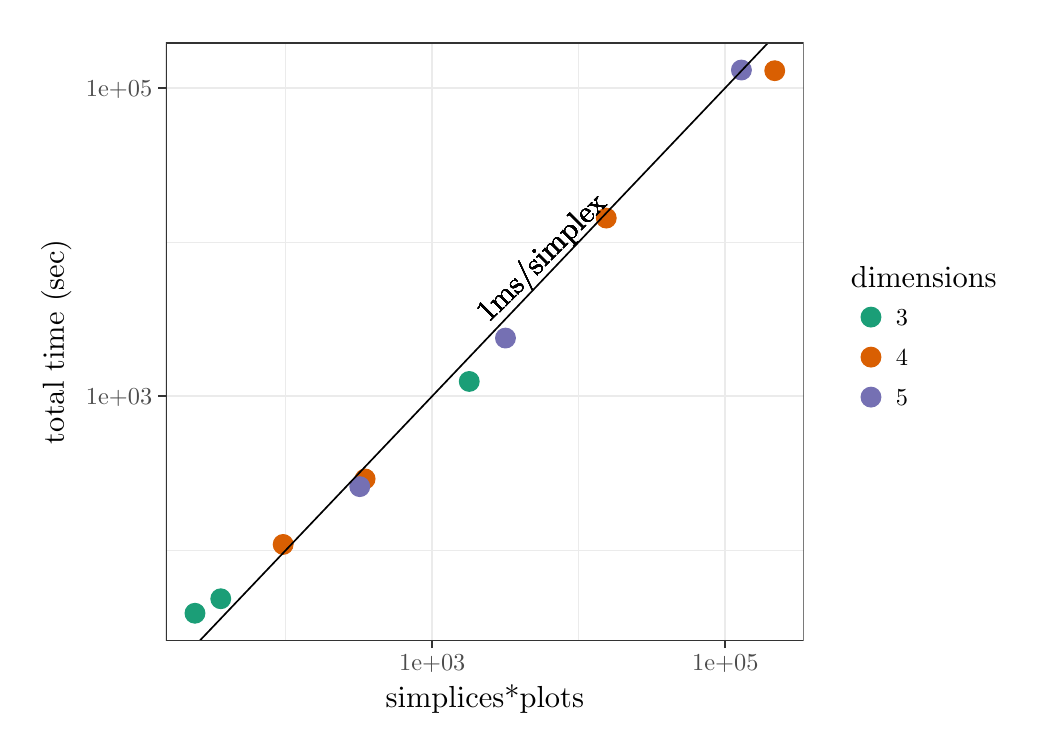
\begin{tikzpicture}[x=1pt,y=1pt]
\definecolor{fillColor}{RGB}{255,255,255}
\path[use as bounding box,fill=fillColor,fill opacity=0.00] (0,0) rectangle (361.35,252.94);
\begin{scope}
\path[clip] (  0.00,  0.00) rectangle (361.35,252.94);
\definecolor{drawColor}{RGB}{255,255,255}
\definecolor{fillColor}{RGB}{255,255,255}

\path[draw=drawColor,line width= 0.6pt,line join=round,line cap=round,fill=fillColor] (  0.00, -0.00) rectangle (361.35,252.94);
\end{scope}
\begin{scope}
\path[clip] ( 49.98, 31.53) rectangle (280.42,247.45);
\definecolor{fillColor}{RGB}{255,255,255}

\path[fill=fillColor] ( 49.98, 31.53) rectangle (280.42,247.45);
\definecolor{drawColor}{gray}{0.92}

\path[draw=drawColor,line width= 0.3pt,line join=round] ( 49.98, 64.13) --
	(280.42, 64.13);

\path[draw=drawColor,line width= 0.3pt,line join=round] ( 49.98,175.51) --
	(280.42,175.51);

\path[draw=drawColor,line width= 0.3pt,line join=round] ( 93.26, 31.53) --
	( 93.26,247.45);

\path[draw=drawColor,line width= 0.3pt,line join=round] (199.14, 31.53) --
	(199.14,247.45);

\path[draw=drawColor,line width= 0.6pt,line join=round] ( 49.98,119.82) --
	(280.42,119.82);

\path[draw=drawColor,line width= 0.6pt,line join=round] ( 49.98,231.20) --
	(280.42,231.20);

\path[draw=drawColor,line width= 0.6pt,line join=round] (146.20, 31.53) --
	(146.20,247.45);

\path[draw=drawColor,line width= 0.6pt,line join=round] (252.08, 31.53) --
	(252.08,247.45);
\definecolor{drawColor}{RGB}{27,158,119}
\definecolor{fillColor}{RGB}{27,158,119}

\path[draw=drawColor,line width= 0.4pt,line join=round,line cap=round,fill=fillColor] ( 69.77, 46.58) circle (  3.57);

\path[draw=drawColor,line width= 0.4pt,line join=round,line cap=round,fill=fillColor] ( 60.45, 41.34) circle (  3.57);
\definecolor{drawColor}{RGB}{217,95,2}
\definecolor{fillColor}{RGB}{217,95,2}

\path[draw=drawColor,line width= 0.4pt,line join=round,line cap=round,fill=fillColor] (121.93, 89.87) circle (  3.57);

\path[draw=drawColor,line width= 0.4pt,line join=round,line cap=round,fill=fillColor] ( 92.32, 66.20) circle (  3.57);
\definecolor{drawColor}{RGB}{117,112,179}
\definecolor{fillColor}{RGB}{117,112,179}

\path[draw=drawColor,line width= 0.4pt,line join=round,line cap=round,fill=fillColor] (172.65,140.78) circle (  3.57);

\path[draw=drawColor,line width= 0.4pt,line join=round,line cap=round,fill=fillColor] (120.00, 87.10) circle (  3.57);
\definecolor{drawColor}{RGB}{217,95,2}
\definecolor{fillColor}{RGB}{217,95,2}

\path[draw=drawColor,line width= 0.4pt,line join=round,line cap=round,fill=fillColor] (269.95,237.39) circle (  3.57);
\definecolor{drawColor}{RGB}{27,158,119}
\definecolor{fillColor}{RGB}{27,158,119}

\path[draw=drawColor,line width= 0.4pt,line join=round,line cap=round,fill=fillColor] (159.56,125.10) circle (  3.57);
\definecolor{drawColor}{RGB}{217,95,2}
\definecolor{fillColor}{RGB}{217,95,2}

\path[draw=drawColor,line width= 0.4pt,line join=round,line cap=round,fill=fillColor] (209.07,184.13) circle (  3.57);
\definecolor{drawColor}{RGB}{117,112,179}
\definecolor{fillColor}{RGB}{117,112,179}

\path[draw=drawColor,line width= 0.4pt,line join=round,line cap=round,fill=fillColor] (257.91,237.63) circle (  3.57);
\definecolor{drawColor}{RGB}{0,0,0}

\path[draw=drawColor,line width= 0.6pt,line join=round] ( 49.98, 18.59) -- (272.75,252.94);

\node[text=drawColor,rotate= 45.00,anchor=base,inner sep=0pt, outer sep=0pt, scale=  1.10] at (188.08,167.42) {1ms/simplex};

\node[text=drawColor,rotate= 45.00,anchor=base,inner sep=0pt, outer sep=0pt, scale=  1.10] at (188.08,167.42) {1ms/simplex};

\node[text=drawColor,rotate= 45.00,anchor=base,inner sep=0pt, outer sep=0pt, scale=  1.10] at (188.08,167.42) {1ms/simplex};

\node[text=drawColor,rotate= 45.00,anchor=base,inner sep=0pt, outer sep=0pt, scale=  1.10] at (188.08,167.42) {1ms/simplex};

\node[text=drawColor,rotate= 45.00,anchor=base,inner sep=0pt, outer sep=0pt, scale=  1.10] at (188.08,167.42) {1ms/simplex};

\node[text=drawColor,rotate= 45.00,anchor=base,inner sep=0pt, outer sep=0pt, scale=  1.10] at (188.08,167.42) {1ms/simplex};

\node[text=drawColor,rotate= 45.00,anchor=base,inner sep=0pt, outer sep=0pt, scale=  1.10] at (188.08,167.42) {1ms/simplex};

\node[text=drawColor,rotate= 45.00,anchor=base,inner sep=0pt, outer sep=0pt, scale=  1.10] at (188.08,167.42) {1ms/simplex};

\node[text=drawColor,rotate= 45.00,anchor=base,inner sep=0pt, outer sep=0pt, scale=  1.10] at (188.08,167.42) {1ms/simplex};

\node[text=drawColor,rotate= 45.00,anchor=base,inner sep=0pt, outer sep=0pt, scale=  1.10] at (188.08,167.42) {1ms/simplex};
\definecolor{drawColor}{gray}{0.20}

\path[draw=drawColor,line width= 0.6pt,line join=round,line cap=round] ( 49.98, 31.53) rectangle (280.42,247.45);
\end{scope}
\begin{scope}
\path[clip] (  0.00,  0.00) rectangle (361.35,252.94);
\definecolor{drawColor}{gray}{0.30}

\node[text=drawColor,anchor=base east,inner sep=0pt, outer sep=0pt, scale=  0.88] at ( 45.03,116.79) {1e+03};

\node[text=drawColor,anchor=base east,inner sep=0pt, outer sep=0pt, scale=  0.88] at ( 45.03,228.17) {1e+05};
\end{scope}
\begin{scope}
\path[clip] (  0.00,  0.00) rectangle (361.35,252.94);
\definecolor{drawColor}{gray}{0.20}

\path[draw=drawColor,line width= 0.6pt,line join=round] ( 47.23,119.82) --
	( 49.98,119.82);

\path[draw=drawColor,line width= 0.6pt,line join=round] ( 47.23,231.20) --
	( 49.98,231.20);
\end{scope}
\begin{scope}
\path[clip] (  0.00,  0.00) rectangle (361.35,252.94);
\definecolor{drawColor}{gray}{0.20}

\path[draw=drawColor,line width= 0.6pt,line join=round] (146.20, 28.78) --
	(146.20, 31.53);

\path[draw=drawColor,line width= 0.6pt,line join=round] (252.08, 28.78) --
	(252.08, 31.53);
\end{scope}
\begin{scope}
\path[clip] (  0.00,  0.00) rectangle (361.35,252.94);
\definecolor{drawColor}{gray}{0.30}

\node[text=drawColor,anchor=base,inner sep=0pt, outer sep=0pt, scale=  0.88] at (146.20, 20.52) {1e+03};

\node[text=drawColor,anchor=base,inner sep=0pt, outer sep=0pt, scale=  0.88] at (252.08, 20.52) {1e+05};
\end{scope}
\begin{scope}
\path[clip] (  0.00,  0.00) rectangle (361.35,252.94);
\definecolor{drawColor}{RGB}{0,0,0}

\node[text=drawColor,anchor=base,inner sep=0pt, outer sep=0pt, scale=  1.10] at (165.20,  7.44) {simplices*plots};
\end{scope}
\begin{scope}
\path[clip] (  0.00,  0.00) rectangle (361.35,252.94);
\definecolor{drawColor}{RGB}{0,0,0}

\node[text=drawColor,rotate= 90.00,anchor=base,inner sep=0pt, outer sep=0pt, scale=  1.10] at ( 13.08,139.49) {total time (sec)};
\end{scope}
\begin{scope}
\path[clip] (  0.00,  0.00) rectangle (361.35,252.94);
\definecolor{fillColor}{RGB}{255,255,255}

\path[fill=fillColor] (291.80,106.52) rectangle (355.85,172.45);
\end{scope}
\begin{scope}
\path[clip] (  0.00,  0.00) rectangle (361.35,252.94);
\definecolor{drawColor}{RGB}{0,0,0}

\node[text=drawColor,anchor=base west,inner sep=0pt, outer sep=0pt, scale=  1.10] at (297.49,159.19) {dimensions};
\end{scope}
\begin{scope}
\path[clip] (  0.00,  0.00) rectangle (361.35,252.94);
\definecolor{fillColor}{RGB}{255,255,255}

\path[fill=fillColor] (297.49,141.12) rectangle (311.95,155.57);
\end{scope}
\begin{scope}
\path[clip] (  0.00,  0.00) rectangle (361.35,252.94);
\definecolor{drawColor}{RGB}{27,158,119}
\definecolor{fillColor}{RGB}{27,158,119}

\path[draw=drawColor,line width= 0.4pt,line join=round,line cap=round,fill=fillColor] (304.72,148.35) circle (  3.57);
\end{scope}
\begin{scope}
\path[clip] (  0.00,  0.00) rectangle (361.35,252.94);
\definecolor{fillColor}{RGB}{255,255,255}

\path[fill=fillColor] (297.49,126.67) rectangle (311.95,141.12);
\end{scope}
\begin{scope}
\path[clip] (  0.00,  0.00) rectangle (361.35,252.94);
\definecolor{drawColor}{RGB}{217,95,2}
\definecolor{fillColor}{RGB}{217,95,2}

\path[draw=drawColor,line width= 0.4pt,line join=round,line cap=round,fill=fillColor] (304.72,133.89) circle (  3.57);
\end{scope}
\begin{scope}
\path[clip] (  0.00,  0.00) rectangle (361.35,252.94);
\definecolor{fillColor}{RGB}{255,255,255}

\path[fill=fillColor] (297.49,112.21) rectangle (311.95,126.67);
\end{scope}
\begin{scope}
\path[clip] (  0.00,  0.00) rectangle (361.35,252.94);
\definecolor{drawColor}{RGB}{117,112,179}
\definecolor{fillColor}{RGB}{117,112,179}

\path[draw=drawColor,line width= 0.4pt,line join=round,line cap=round,fill=fillColor] (304.72,119.44) circle (  3.57);
\end{scope}
\begin{scope}
\path[clip] (  0.00,  0.00) rectangle (361.35,252.94);
\definecolor{drawColor}{RGB}{0,0,0}

\node[text=drawColor,anchor=base west,inner sep=0pt, outer sep=0pt, scale=  0.88] at (313.75,145.32) {3};
\end{scope}
\begin{scope}
\path[clip] (  0.00,  0.00) rectangle (361.35,252.94);
\definecolor{drawColor}{RGB}{0,0,0}

\node[text=drawColor,anchor=base west,inner sep=0pt, outer sep=0pt, scale=  0.88] at (313.75,130.86) {4};
\end{scope}
\begin{scope}
\path[clip] (  0.00,  0.00) rectangle (361.35,252.94);
\definecolor{drawColor}{RGB}{0,0,0}

\node[text=drawColor,anchor=base west,inner sep=0pt, outer sep=0pt, scale=  0.88] at (313.75,116.41) {5};
\end{scope}
\end{tikzpicture}

  }
  \caption{%
    Chart showing the number of slicing operations 
    (simplices $\times$ number of plots) versus timing results from running 
    our algorithm on a number of different datasets. The axes are on a log-log
    scale. The points are all clustered around the ``1 ms/simplex'' line 
    showing that the running time is roughly one millisecond per slicing 
    operation.
  }
  \label{fig:timing}
\end{figure}

In order to test the running time of the slicing algorithm I ran a number of
experiments to understand the timing. I tested regular polytopes in 3, 4, and
5 dimensions as well as hyperspheres. I also tested the four-dimensional
version of the Klein bottle because it has a large number of simplices in its
mesh. For each test, I ran the slicing algorithm for all pairs of dimensions
and for $1,000$ focus points. I recorded the total wall clock time as well as
the number of simplices given by the quickhull algorithm. The testing machine
has an 8-core 3.2GHz Intel i7-6900K with 64GB of RAM.

The results are shown in \autoref{tbl:timings}. The total number of slicing
checks (\autoref{alg:slicing:single}) is the number of simplices, times the
number of pairs of dimensions ($d \choose 2$), times the total number of focus
points ($1,000$). I divide the total time by this number to show the time per
simplex. 

As we can see, the times are roughly constant between the number of
dimensions and simplices (see \autoref{fig:timing}). The reason the Klein 
bottle is faster is because
many slices do not hit any simplices and the algorithm will exit early
once this is detected. Right now this algorithm is not optimized.
For example, it would be greatly beneficial to pre-compute a spatial data
structure so that only slices that are likely to intersect simplices are
evaluated. Currently, the algorithm must check every simplex against every
focus point for every pair of dimensions. This is a lot of extra work for figures
such as the Klein bottle with many simplexes.


\section{Limitations and future work}

In this paper we have presented the characteristics of data used for
analyzing computer simulations under the 
\emph{design and analysis of computer experiments} 
framework~\cite{Santner:2003}.  We investigate
how interactive rendering times may be used in this framework using the
HyperSlice~\cite{Wijk:1993} rendering technique implemented on the GPU.
We then describe a method using both the scene geometry and estimates of the
user's machine capabilities in order to make an accurate prediction of 
the rendering time.
We find that timing, especially using wall-clock time, is extremely noisy
and makes fitting very difficult.  It is much more reliable to use the
timer on the GPU itself, however one must take into account the time needed
to return back from the GPU which in our experiments is about 1ms.

In the future, we will investigate how to reduce the number of trials
needed to properly fit the formula.  Currently each dimension
takes about 6 hours to complete and requires the machine to be dedicated
to running the timing code.  Reducing the number of trials will help to
alleviate this time consuming task.

It would also be interesting to extend our approach to the analysis of
HyperSlice rendering in general. The basic geometrical operation in our
mathematical model is slicing multi-dimensional spheres with 2D planes and
estimating the area. Therefore our method should work directly with any radial
basis function reconstruction technique like the work by Hong et
al.~\cite{Hong:2006} although we have not directly tested this.  We would also
like to extend our mathematical model to take the shape of the reconstruction
primitive into account. This would allow us to analyze the timing of HyperSlice
rendering using a much more broad set of reconstruction methods like 
nearest neighbor or linear regression. 
The framework can also be used to estimate the rendering time of density
estimation by setting $f(x_i) = 1$ in \autoref{eq:kernel_regression}. Repeating the
analysis using box primitives would allow us to estimate the time complexity
of some of the recent real-time large-data aggregation and visualization 
methods like imMens~\cite{Liu:2013} and NanoCubes~\cite{Lins:2013}. Both these
methods use rectangular binning in their density estimation.

We will also implement our subsampling strategy.
There is a lot of overdrawing occurring which does not contribute at
all to the final plot as the color channel is effectively maxed out, 
especially as the value of $N$ and $r$ increases.  By detecting when this 
occurs and only rendering the first few points we could improve rendering
efficiency.



